\documentclass[a4paper,9pt,twocolumn]{jsarticle}

\usepackage[
  a4paper,
  top=20mm,
  bottom=20mm,
  left=20mm,
  right=20mm,
  includehead=false,
  includefoot=false
]{geometry}


\usepackage[dvipdfmx]{graphicx}
\usepackage{amsmath,amssymb}
\usepackage{bm}
\usepackage{newtxtext}
\usepackage{newtxmath}
\usepackage{booktabs}
\usepackage{url}
\usepackage{caption}
\usepackage{subcaption}
\usepackage{titlesec}
\usepackage{enumitem}
\usepackage{tikz}
\usetikzlibrary{
  positioning,
  arrows.meta,
  shapes.geometric,
  fit,
  calc
}

\setlength{\columnsep}{2zw}
\setlength{\columnseprule}{0pt}

\AtBeginDocument{%
  \mcfamily
  \fontsize{9pt}{14.4pt}\selectfont
}

\titleformat{\section}
  {\gtfamily\fontsize{10pt}{14.4pt}\selectfont\bfseries}
  {\thesection.}{0.5zw}{}
\titlespacing*{\section}
  {0pt}{14.4pt}{0pt}

\titleformat{\subsection}
  {\gtfamily\fontsize{9pt}{14.4pt}\selectfont\bfseries}
  {\thesubsection}{0.5zw}{}
\titlespacing*{\subsection}
  {0pt}{0pt}{0pt}

\titleformat{\subsubsection}
  {\gtfamily\fontsize{9pt}{14.4pt}\selectfont\bfseries}
  {\thesubsubsection}{0.5zw}{}
\titlespacing*{\subsubsection}
  {0pt}{0pt}{0pt}

\DeclareCaptionFont{jagothic}{%
  \gtfamily\fontsize{9pt}{11pt}\selectfont
}
\captionsetup{
  font=jagothic,
  labelfont=jagothic,
  labelsep=colon,
  justification=centering
}
\captionsetup[table]{position=top}
\setlength{\abovecaptionskip}{4pt}
\setlength{\belowcaptionskip}{4pt}

\setlist[itemize]{
  leftmargin=1.5zw,
  itemsep=0pt,
  parsep=0pt,
  topsep=2pt
}

\pagestyle{empty}
\setlength{\parindent}{1zw}
\setlength{\parskip}{0pt}
\renewcommand{\refname}{\centering\gtfamily\fontsize{10pt}{14.4pt}\selectfont 参考文献}

\begin{document}

\twocolumn[
\begin{center}

\vspace*{-8mm}

{\gtfamily\fontsize{18pt}{22pt}\selectfont\bfseries
MirrorForm：身体感覚を可視化するMRパーソナルトレーナー
\par}

\vspace{1\baselineskip}

{\rmfamily\fontsize{10pt}{12pt}\selectfont
MirrorForm: An MR Personal Trainer for Visualizing Exercise Form
\par}

\vspace{1\baselineskip}

{\mcfamily\fontsize{10pt}{12pt}\selectfont
吉田 智昭
\par}

{\rmfamily\fontsize{10pt}{12pt}\selectfont
Tomoaki YOSHIDA
\par}

\vspace{1\baselineskip}

{\mcfamily\fontsize{9pt}{11pt}\selectfont
東京大学大学院 情報理工学系研究科 コンピュータ科学専攻\\
（〒113--8656 東京都文京区本郷7--3--1,
\texttt{yoshida-tomoaki855@g.ecc.u-tokyo.ac.jp}）
\par}

\vspace{1\baselineskip}

\begin{minipage}{\dimexpr\textwidth-10zw\relax}
\rmfamily\fontsize{9pt}{11pt}\selectfont
\textbf{Abstract:}
This paper proposes MirrorForm, an MR-based personal training system that visualizes differences between a user's exercise form and a target form.
The envisioned system estimates three-dimensional body posture using multiple cameras and presents corrective feedback through an MR headset.
As a first prototype, we implemented a single-camera squat analysis system using MediaPipe Pose.
The prototype detects squat repetitions, evaluates six form-related indicators, and visualizes the results through an annotated video and an analysis report.
In a test video containing 15 squat repetitions, the system detected all 15 repetitions and generated feedback for each repetition.

\medskip
\textbf{\textit{Key Words:}}
\textit{Mixed Reality, Pose Estimation, Personal Training, Form Visualization}
\end{minipage}

\end{center}

\vspace{2\baselineskip}
]

\section{はじめに}

筆者は日常的に筋力トレーニングを行っているが, 一人でトレーニングする際, 自分のフォームを正確に把握することが難しいと感じている. 
自分では正しい姿勢を取っているつもりでも, 後から撮影動画を確認すると, 腰の反りや体幹の傾き, スクワットの深さなどに問題が見つかることがある. 
実際に視覚的なフィードバックは, 初心者によるスクワット動作の習得や保持を支援する可能性が報告されている\cite{shin_feedback}. 
しかし, セットごとにスマートフォンを設置し, 運動後に動画を見返す作業は煩雑であり, その場で姿勢を修正することもできない. 

また, 一人で行うトレーニングは単調であり, 限界付近まで自分を追い込むための動機を保つことも難しい. 
筆者自身, 好みの声, 特に異性の声で「あと1回」「まだいけます」と応援されると, 普段よりも力を出せるように感じる. 
そこで, フォームを冷静に分析するだけでなく, 利用者の好みに合わせた姿や声を持つ仮想トレーナーが, すぐ近くから応援してくれる環境が欲しいと考えた. 

本稿では, 複数視点カメラと複合現実感（MR）を用いて, 利用者のフォームをリアルタイムに解析し, 理想フォームとの差を視覚的に提示するMRパーソナルトレーナー「MirrorForm」を提案する. 
本システムは, 数回のスクワットを確認し, 一人で行うトレーニングを少し楽しくするためだけに, 複数カメラ, 三次元姿勢推定, MR表示, 音声エージェントを投入する, 個人的な欲望に忠実な「技術の無駄遣い」である. 

さらに, 提案システムの第一段階として, 単一RGBカメラからスクワットフォームを解析し, 警告付き動画と反復ごとの評価レポートを生成するプロトタイプを実装した. 

\section{提案システム}

\subsection{システム概要}

提案システムでは, 利用者の正面および側面に設置した複数台のカメラから身体姿勢を推定し, 三次元骨格情報を取得する. 
得られた姿勢を種目ごとの理想フォームと比較し, 関節角度や身体各部の位置関係の違いを算出する. 

解析結果はMRヘッドセット上に重畳表示され, 現在のフォーム, 理想フォーム, 修正すべき部位を直感的に確認できる. 
また, 音声エージェントがリアルタイムでアドバイスや励ましを行うことで, パーソナルトレーナーと共にトレーニングしているような体験を提供する. 
\begin{figure*}[bt]
    \centering
    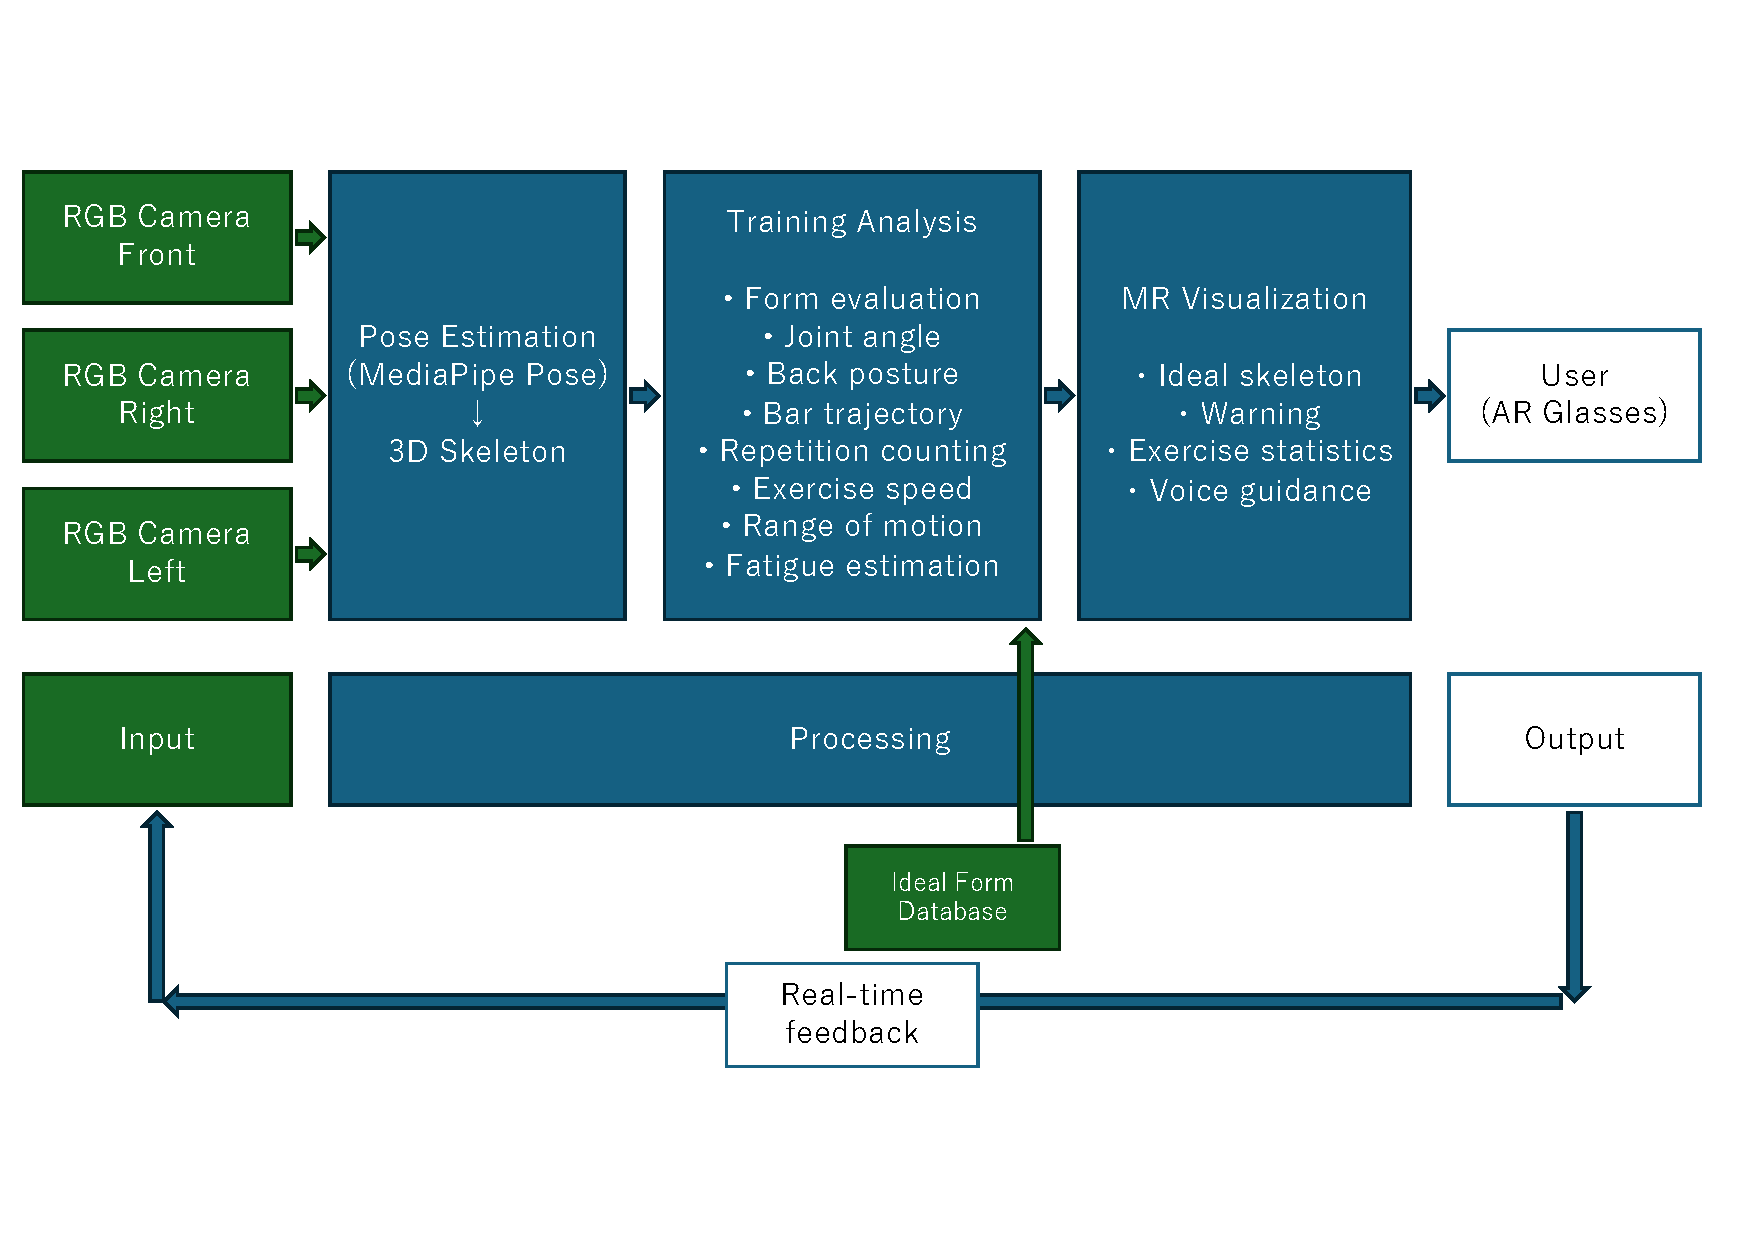
\includegraphics[
        width=0.96\textwidth,
        trim=10 80 10 80,
        clip
    ]{figures/figure1.pdf}
    \caption{
    提案するMRパーソナルトレーナーのシステム概要. 
    複数視点のRGBカメラから利用者の三次元姿勢を推定し, 理想フォームデータベースと比較して, フォーム, 回数, 動作速度, 疲労状態などを解析する. 
    解析結果はMR表示および音声ガイダンスとして提示され, 利用者はリアルタイムにフォームを修正できる. 
    なお, 複数視点による三次元姿勢復元, 疲労推定, MR表示, 音声ガイダンスは将来機能であり, 本プロトタイプでは実装していない. 
    }
    \label{fig:system_overview}
\end{figure*}

\subsection{得られる体験}

本システムでは, 利用者はトレーニング中にMRヘッドセットを装着するだけで, 自分のフォームと理想フォームとの差をリアルタイムに確認できる. 

例えばベンチプレスでは, 現在の姿勢に半透明の理想フォームを重ねて表示し, 腰椎の過伸展, 胸椎の伸展不足, バー軌道のずれなどを色分けして提示する. 
スクワットでは膝や股関節の角度, デッドリフトでは背中の丸まりなど, 種目ごとに重要な部位を可視化する. 
これにより, 「胸を張る」「腰を反らさない」といった言葉だけでは理解しにくい指示を, 身体のどの部分をどの方向へ動かせばよいかという視覚情報として理解できる. 

さらに, 本システムでは, 利用者の好みに合わせた外見や声を持つ仮想トレーナーをMR空間に提示する. 
仮想トレーナーは, 「あと少し深くしゃがんでください」といったフォーム修正に加え, 「あと1回です」「まだいけます」といった応援を行う. 
声の性別, 話し方, 励ましの強さなどを利用者が選択できるため, 厳しいコーチ, 落ち着いた指導者, 親しい友人のような話し方など, 利用者が最も意欲を保ちやすい体験を設定できる. 
利用者の好みに応じて外見や声を変更できるため, 一般的な音声アシスタントよりも親近感を持ちやすく, 継続や努力を促す効果が期待できる. 

\subsection{利用シーン}

本システムは, 自宅やジムにおける筋力トレーニングを対象とする. 

利用者はMRヘッドセットを装着した状態でトレーニングを行う. 
トレーニング中は, 現在のフォームと理想フォームとの差異がリアルタイムに表示されるため, 鏡を見なくても姿勢を修正できる. 

また, トレーニング終了後には, 各セットのフォームを自動で記録し, 改善点や過去との比較を確認できる. 
これにより, 継続的なフォーム改善を支援する. 

\section{プロトタイプ実装}

提案システム全体を実現するためには, 複数台カメラを用いた三次元姿勢推定, MRヘッドセットへの描画, 音声エージェントとの連携など, 多数の要素技術が必要となる. 
そこで本研究では, 提案システムの実現可能性を確認する第一段階として, 単一RGBカメラを用いたフォーム解析プロトタイプを実装した. 

本プロトタイプでは, 人体姿勢推定による骨格取得, フォーム評価, および評価結果の可視化機能を実装対象とした. 
一方, MR空間への重畳表示や複数視点による三次元姿勢復元については, 将来的な拡張機能として位置付ける. 

本プロトタイプのソースコード, 実行方法, および出力例は, 
GitHub上で公開している\footnote{
\url{https://github.com/tomoaki855/mixed_reality2026}
}. 

\subsection{姿勢推定}

人体姿勢推定にはMediaPipe Poseを用いた. 
MediaPipe Poseの姿勢推定器はBlazePoseを基礎とし, 単一人物の33点の身体ランドマークをリアルタイムに推定する\cite{mediapipe,blazepose}. 
本プロトタイプでは肩, 耳, 股関節, 膝, 足首などのランドマークを利用した. 

撮影は利用者の側面から単一RGBカメラで行い, 各フレームについて姿勢推定を実行する. 
推定されたランドマーク座標を用いて, 関節角度や体幹姿勢など, フォーム評価に必要な各種特徴量を算出する. 

提案システムでは, 正面・左右など複数方向に配置したカメラ画像を用いることを想定している. 
各カメラの内部・外部パラメータを事前にキャリブレーションした後, 対応するランドマークを三角測量によって統合することで, 三次元姿勢を復元する予定である. 

\subsection{フォーム評価}

本プロトタイプでは, スクワットフォームを評価するために, 膝関節角度, 股関節角度, 体幹前傾角度, スクワット深さ, 上背部の丸まり, 足部バランスの6項目を評価対象とした. 

膝関節角度および股関節角度は, MediaPipe Poseによって推定されたランドマーク座標から算出する. 
また, 体幹前傾角度は肩と股関節を結ぶベクトルと鉛直方向とのなす角として定義し, スクワット中の過度な前傾姿勢を検出するために用いた. 

スクワット深さについては, 利用者の体格による影響を低減するため, 
股関節と膝の鉛直方向の位置差を下腿長で正規化した指標を導入した. 
深さ指標 $D$ は

\begin{equation}
D=
\frac{
y_{\mathrm{hip}}-y_{\mathrm{knee}}
}{
\left\|
\mathbf{p}_{\mathrm{knee}}
-
\mathbf{p}_{\mathrm{ankle}}
\right\|
}
\end{equation}

で定義する. 
ここで, 
$y_{\mathrm{hip}}$, 
$y_{\mathrm{knee}}$
はそれぞれ股関節および膝の画像座標における鉛直位置, 
$\mathbf{p}_{\mathrm{knee}}$, 
$\mathbf{p}_{\mathrm{ankle}}$
は膝および足首の2次元位置ベクトルを表す. 
分母で下腿長を用いて正規化することで, 身長や撮影距離の違いによる影響を低減している. 

また, 上背部の丸まりは, 耳・肩・股関節から算出した上半身角度を基準姿勢と比較することで評価した. 
スクワット開始時の姿勢を基準角度 $\theta_{\mathrm{neutral}}$ とし, 現在の上半身角度を $\theta_{\mathrm{current}}$ とすると, 丸まり量は

\begin{equation}
\Delta\theta
=
\theta_{\mathrm{neutral}}
-
\theta_{\mathrm{current}}
\end{equation}

として表される. 
$\Delta\theta$ が大きいほど, 上背部が屈曲していると判断する. 

さらに, 股関節位置と踵・つま先位置との相対関係から, 前後方向の姿勢バランスを近似的に評価した. 
足部バランス指標 $R$ を

\begin{equation}
R=\frac{x_{\mathrm{hip}}-x_{\mathrm{heel}}}{x_{\mathrm{toe}}-x_{\mathrm{heel}}}
\end{equation}

と定義する. 
ここで, $x_{\mathrm{hip}}$, $x_{\mathrm{heel}}$, $x_{\mathrm{toe}}$はそれぞれ股関節, 踵, つま先の水平方向座標である. 
$R$ が小さい場合は股関節の投影位置が踵側にあり, 大きい場合はつま先側にあると判定する. 
本指標は実際の身体重心や足圧中心を計測するものではなく, 画像上の位置関係から前後方向の姿勢傾向を近似的に表す指標である. 

本プロトタイプでは動作確認を目的として, 各評価指標に対する閾値を経験的に設定した. 
基準を満たさない場合には, 対応する警告メッセージを表示する. 
また, 膝関節角度の変化からスクワット動作を自動的に1回ごとへ分割し, 各反復に対して総合的なフォーム評価を実施することで, 利用者が修正すべきポイントを直感的に把握できるようにした. 

\subsection{実装結果}

\begin{figure*}[tb]
    \centering
    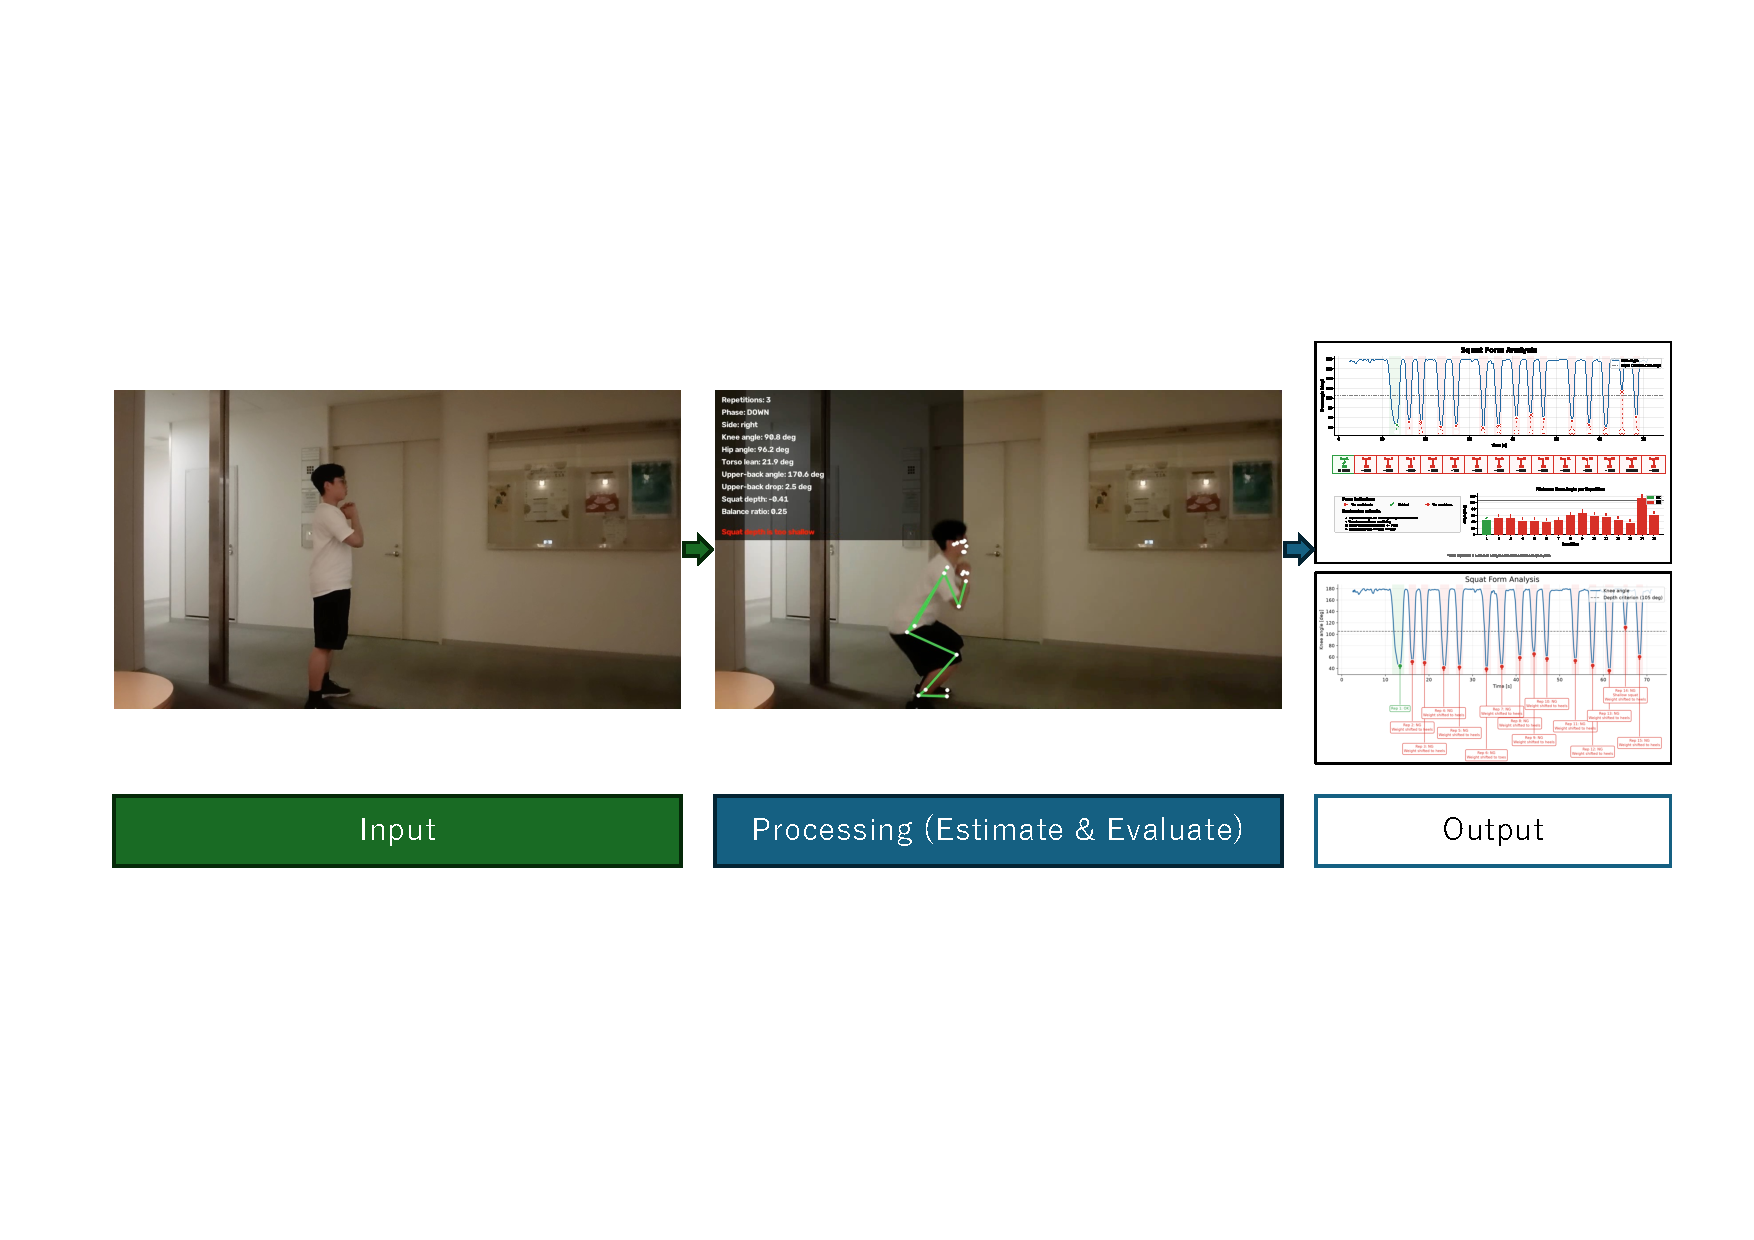
\includegraphics[
        width=\textwidth,
        trim=30 150 30 130,
        clip
    ]{figures/prototype_pipeline.pdf}
    \caption{
    実装したスクワットフォーム解析プロトタイプの処理例. 
    入力動画に対して人体姿勢推定を行い, 推定された骨格情報から関節角度, スクワット深さ, 体幹姿勢, 足部バランスなどを評価する. 
    処理結果は入力映像上への骨格および警告表示と, 反復ごとの評価結果をまとめた解析レポートとして出力される. 
    }
    \label{fig:prototype_pipeline}
\end{figure*}

実装したプロトタイプの処理例を図\ref{fig:prototype_pipeline}に示す. 
入力されたスクワット動画の各フレームに対してMediaPipe Poseによる姿勢推定を実行し, 推定されたランドマーク上に骨格を描画する. 

同時に, 膝関節角度, 股関節角度, 体幹前傾角度, 上背部の丸まり, スクワット深さ, 足部バランスを算出し, 設定した基準を満たさない場合には, 映像上に警告メッセージを表示する. 
図中の例では, スクワット最深部において深さが不足していると判定され, ``Squat depth is too shallow''という警告が表示されている. 

また, 膝関節角度の時系列変化からスクワット動作を1回ごとに分割し, 各反復についてフォーム評価を行う. 
解析終了後には, 膝関節角度の推移, 各反復の最深部, OK/NG判定, および警告内容をまとめたレポートを生成する. 

これにより, 利用者は動画全体を見返さなくても, どの反復で, どのようなフォームの崩れが生じたかを確認できる. 

\section{評価}

実装したプロトタイプについて, スクワット動画を入力し, 姿勢推定, 反復回数の検出, フォーム評価, 警告表示, 解析レポート生成が一連の処理として動作するかを確認した. 

評価には, 側面から撮影したスクワット動画を用いた. 
動画中には目視で15回のスクワット動作が含まれており, 本プロトタイプも膝関節角度の周期的な変化に基づいて15回の反復を検出した. 

各反復について, 膝関節角度, 股関節角度, 体幹前傾角度, 上背部の丸まり, スクワット深さ, 足部バランス指標を算出し, 設定した閾値を満たさない場合には警告を出力した. 
また, 入力映像上へ骨格および警告を重畳した動画と, 各反復の最深部, OK/NG判定, 警告内容をまとめた解析レポートを生成できることを確認した. 

以上より, 単一のRGB動画を入力として, 姿勢推定から反復検出, フォーム指標の算出, 結果の可視化までを自動的に実行できることを確認した. 
ただし, 本評価では各警告が専門的なフォーム判定と一致するかは検証していない. 
そのため, 本評価は判定精度を示すものではなく, プロトタイプの一連の機能が動作することを確認するための動作評価として位置付ける. 

\section{考察}

評価結果より, 単一のRGBカメラで撮影した動画から, スクワットの反復回数を自動的に検出し, 各反復に対して複数のフォーム指標を算出できることを確認した. 
また, 入力映像への警告表示と解析レポートの生成を組み合わせることで, 利用者がフォームの崩れを視覚的に確認できるプロトタイプを実現できた. 

特に, 本システムでは「背中を丸めない」「深くしゃがむ」といった言語だけでは理解しにくい指示を, 関節角度や身体位置に基づく数値および警告として提示できる. 
将来的にこれらをMR空間へ重畳表示することで, 利用者は鏡や撮影動画に視線を移すことなく, トレーニング中にその場でフォームを修正できると考えられる. 

一方, 本プロトタイプにはいくつかの制約がある. 
第一に, 単一カメラによる二次元姿勢推定では, 奥行き方向の動きや身体のひねりを正確に取得することが難しい. 
また, 腕や脚が身体と重なる自己遮蔽や, 利用者が撮影範囲から外れた場合には, ランドマーク推定が不安定になる可能性がある. 
今後は, 正面および左右に配置した複数カメラを用いて三次元姿勢を復元することで, これらの問題を軽減する必要がある. 

第二に, 本実装におけるフォーム評価は, あらかじめ設定した閾値に基づいている. 
しかし, 適切なスクワットフォームは, 利用者の身長, 骨格, 柔軟性, トレーニング経験, および目的によって異なる. 
そのため, 全利用者に同一の閾値を適用すると, 安全なフォームを誤って警告したり, 危険なフォームを見逃したりする可能性がある. 
今後は, 利用開始時に基準姿勢や可動域を計測し, 利用者ごとに判定基準を調整する仕組みが必要である. 

第三に, 本実装で用いた足部バランス指標は, 股関節と踵・つま先の画像上の位置関係を利用した近似であり, 実際の足圧中心や身体重心を直接計測したものではない. 
したがって, 「踵側に偏っている」「つま先側に偏っている」という警告は, 身体の前後方向の姿勢傾向を表す参考情報として扱う必要がある. 
より正確な評価には, 足圧センサや床反力計との組合せが有効であるが, 装置が増えることで手軽さが失われるという欠点もある. 

また, 現在のプロトタイプは撮影済み動画を解析する方式であり, MRデバイス上でのリアルタイム表示は実装していない. 
リアルタイム化に際しては, 姿勢推定から警告表示までの遅延, 視野内に表示する情報量, トレーニング中の視認性などを検討する必要がある. 
警告を過剰に表示すると運動への集中を妨げる可能性があるため, 重大なフォームの崩れだけを短い音声や色で提示し, 詳細な分析はセット終了後に表示する方法が適切だと考えられる. 
また, 仮想トレーナーによる応援は, 利用者の意欲を高める可能性がある一方で, 過度な運動を促す危険もある. 
利用者が好む外見や声を持つ存在から励まされることで, 本来中止すべき状態でも運動を継続してしまう可能性がある. 
そのため, 将来的にはフォームの大きな崩れ, 動作速度の低下, 反復回数などを用いて疲労状態を推定し, 危険がある場合には応援ではなく休憩を促す設計が必要である. 

以上より, 本プロトタイプは, MirrorFormの中心となる姿勢解析およびフォーム可視化の基本機能を実現したものといえる. 
一方で, 判定基準の妥当性や実際のフォーム改善効果については未検証である. 
今後は, トレーナーによる判定との比較や, 鏡を用いた場合, 動画を後から確認する場合, MRによるリアルタイム提示を行う場合の比較実験を実施し, 提案システムの有効性を評価する必要がある. 

\section{おわりに}

本稿では, 筋力トレーニング中の身体感覚を可視化するMRパーソナルトレーナー「MirrorForm」を提案した. 
提案システムでは, 複数視点カメラによる三次元姿勢推定とMR表示を組み合わせることで, 現在のフォームと理想フォームの差異を利用者へ直感的に提示する. 

また, 提案システムの第一段階として, 単一RGBカメラを用いたスクワットフォーム解析プロトタイプを実装した. 
評価動画から15回のスクワット動作を自動的に検出し, 各反復について関節角度, スクワット深さ, 体幹姿勢, 上背部の丸まり, および前後方向の姿勢バランス指標を算出できることを確認した. 
さらに, 警告付き動画と反復ごとの解析レポートを生成することで, 利用者がフォームの崩れを振り返るための基本機能を実現した. 

今後は, 複数視点からの三次元姿勢復元, 利用者の体格や可動域に応じた判定基準の個人化, およびMRデバイス上でのリアルタイム提示を実装する. 
さらに, トレーナーによる判定や従来の鏡・動画確認との比較を通じて, フォーム改善への有効性と提示方法の使いやすさを評価したい. 

\vspace{\baselineskip}

\begin{thebibliography}{9}
\fontsize{9pt}{11pt}\selectfont
\bibitem{shin_feedback}
H.-J. Shin, S.-H. Kim, and H.-Y. Cho:
``The Effect of Types of Sensory Feedback on the Acquisition and Retention of Squat Performance:
A Randomized, Double-Blind, Controlled Trial,''
Scandinavian Journal of Medicine \& Science in Sports,
Vol.~34, No.~1, e14531, 2024.
\bibitem{mediapipe}
C. Lugaresi et al.:
``MediaPipe: A Framework for Building Perception Pipelines,''
arXiv preprint arXiv:1906.08172, 2019.
\bibitem{blazepose}
V. Bazarevsky, I. Grishchenko, K. Raveendran, T. Zhu, F. Zhang, and M. Grundmann:
``BlazePose: On-device Real-time Body Pose Tracking,''
arXiv preprint arXiv:2006.10204, 2020.
\end{thebibliography}

\end{document}
